% Metódy inžinierskej práce

\documentclass[10pt,twocolumn,twoside,slovak,a4paper]{article}

\usepackage[slovak]{babel}
%\usepackage[T1]{fontenc}
\usepackage[IL2]{fontenc} % lepšia sadzba písmena Ľ než v T1
\usepackage[utf8]{inputenc}
\usepackage{graphicx}
\usepackage{url} % príkaz \url na formátovanie URL
\usepackage{hyperref} % odkazy v texte budú aktívne (pri niektorých triedach dokumentov spôsobuje posun textu)

\usepackage{cite}
%\usepackage{times}

\pagestyle{headings}

\title{Algoritmy na hľadanie najkratšej cesty v navigačných systémoch\thanks{Semestrálny projekt v predmete Metódy inžinierskej práce, ak. rok 2024/25, vedenie: Yehveniia Kataieva}} % meno a priezvisko vyučujúceho na cvičeniach

\author{Peter Martišovič\\[2pt]
	{\small Slovenská technická univerzita v Bratislave}\\
	{\small Fakulta informatiky a informačných technológií}\\
	{\small \texttt{xmartisovic@stuba.sk}}
	}

\date{\small 26. september 2024} % upravte


\usepackage{wrapfig}
\usepackage{amsmath}

\begin{document}

\maketitle

\begin{abstract}
\ldots
\end{abstract}



\section{Úvod}

Tento článok sa zameriava na výskum a analýzu algoritmov, ktoré využívajú moderné navigačné systémy, napríklad Waze, Sygic či Google Maps. Algoritmy zohrávajú v navigačných systémoch kľúčovú úlohu na nájdenie tej najkratšej a najrýchlejšej možnej cesty medzi dvomi bodmi. Tieto algoritmy zohľadňujú pri svojom rozhodovaní rôzne faktory, ako sú vzdialenosť, meteorologické podmienky alebo dopravná situácia ako napríklad zápchy či aktuálne nehody. Najdôležitejší je pritom čas cesty, keďže väčšina navigačných systémov sa snaží používateľom odporúčať najrýchlejšiu možnú cestu.

Medzi najznámejšie algoritmy, ktoré sa využívajú pri tvorbe navigačných systémov, patrí Dijkstrov algoritmus a A* algoritmus. Tento článok sa zameriava na analýzu týchto dvoch algoritmov a porovnáva ich použitie v reálnom živote.

Na téme tohto článku som sa rozhodol pracovať preto, lebo chcem zistiť viac informácií o tom, ako fungujú dnešné navigačné systémy. Väčšina ľudí, ktorí ich používajú ani netušia, aké komplexné procesy prebiehajú v pozadí aplikácie pri hľadaní ideálnej trasy. Pochopenie fungovania algoritmov nás môže nielen obohatiť, ale súčasne pri ňom môžeme zistiť, akým spôsobom samy prispievame k efektívnejšiemu plánovaniu trás.

Primárnym zdrojom pre tento článok je publikácia dostupná na IEEE, ktorá skúma pokročilé algoritmy pre výpočet najkratšej trasy a ich implementáciu v reálnych systémoch. Článok čerpá aj z ďalších vedeckých zdrojov zameraných na algoritmy hľadajúce najkratšiu možnú cestu medzi dvomi bodmi.

Základný problém, ktorý bol naznačený v úvode, je podrobnejšie vysvetlený v časti~\ref{nejaka}.
Dôležité súvislosti sú uvedené v častiach~\ref{dolezita} a~\ref{dolezitejsia}.
Záverečné poznámky prináša časť~\ref{zaver}.



\begin{figure}[h]
  \centering
  
\includegraphics[width=0.3\textwidth]{logofiit.png}
\end{figure}

\section{Navigačné systémy} \label{nejaka}

Z obr.~\ref{f:rozhod} je všetko jasné. 


\begin{multline}
d_1 + d_2 + d_3 + \cdots + d_n = \\
\sum_{i=1}^{n} d_i = n \times d
\end{multline}

\[ %matica
\mathbf{A} = \begin{bmatrix}
a_{11} & a_{12} & a_{13} & a_{14} \\
a_{21} & a_{22} & a_{23} & a_{24} \\
a_{31} & a_{32} & a_{33} & a_{34} \\
a_{41} & a_{42} & a_{43} & a_{44} \\
a_{51} & a_{52} & a_{53} & a_{54}
\end{bmatrix}
\]



\begin{figure*}[tbh]
\centering
%\includegraphics[scale=1.0]{diagram.pdf}
Aj text môže byť prezentovaný ako obrázok. Stane sa z neho označný plávajúci objekt. Po vytvorení diagramu zrušte znak \texttt{\%} pred príkazom \verb|\includegraphics| označte tento riadok ako komentár (tiež pomocou znaku \texttt{\%}).
\caption{Rozhodujúci argument.}
\label{f:rozhod}
\end{figure*}




\section{Najkratšia cesta} \label{najkratsiaCesta}

Navigačné systémy sa snažia nájsť čo najkratšiu cestu, ako vidíme aj v Obrázku č. ~\ref{fig:hladanieNajkratsejCesty}
\begin{figure*}[h!]
\centering
  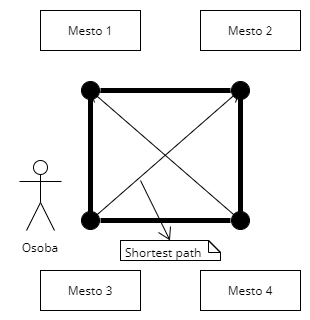
\includegraphics[scale=0.6]{graf1.png}
  \caption{Hľadanie najkratšej cesty}
  \label{fig:hladanieNajkratsejCesty}
\end{figure*}
\begin{figure*}[h!]
\centering
  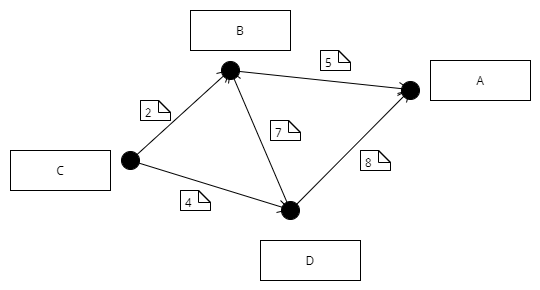
\includegraphics[scale=0.4]{graf2.png}
  \caption{A* algoritmus}
  \label{fig:hladanieNajkratsejCesty}
\end{figure*}


\section{Iná časť} \label{ina}

Základným problémom je teda\ldots{} Najprv sa pozrieme na nejaké vysvetlenie (časť~\ref{ina:nejake}), a potom na ešte nejaké (časť~\ref{ina:nejake}).\footnote{Niekedy môžete potrebovať aj poznámku pod čiarou.}

Môže sa zdať, že problém vlastne nejestvuje\cite{Coplien:MPD}, ale bolo dokázané, že to tak nie je~\cite{Czarnecki:Staged, Czarnecki:Progress}. Napriek tomu, aj dnes na webe narazíme na všelijaké pochybné názory\cite{PLP-Framework}. Dôležité veci možno \emph{zdôrazniť kurzívou}.


\subsection{Nejaké vysvetlenie} \label{ina:nejake}

Niekedy treba uviesť zoznam:

\begin{itemize}
\item jedna vec
\item druhá vec
	\begin{itemize}
	\item x
	\item y
	\end{itemize}
\end{itemize}

Ten istý zoznam, len číslovaný:

\begin{enumerate}
\item jedna vec
\item druhá vec
	\begin{enumerate}
	\item x
	\item y
	\end{enumerate}
\end{enumerate}


\subsection{Ešte nejaké vysvetlenie} \label{ina:este}

\paragraph{Veľmi dôležitá poznámka.}
Niekedy je potrebné nadpisom označiť odsek. Text pokračuje hneď za nadpisom.



\section{Dôležitá časť} \label{dolezita}




\section{Ešte dôležitejšia časť} \label{dolezitejsia}




\section{Záver} \label{zaver} % prípadne iný variant názvu



%\acknowledgement{Ak niekomu chcete poďakovať\ldots}


% týmto sa generuje zoznam literatúry z obsahu súboru literatura.bib podľa toho, na čo sa v článku odkazujete
\bibliography{literatura}
\bibliographystyle{abbrv} % prípadne alpha, abbrv alebo hociktorý iný
\end{document}
